\documentclass[]{article}

\usepackage{amsmath}
\usepackage{bbm}
\usepackage{xcolor}
\usepackage{graphicx}
\graphicspath{ {./figs/} }

\newcommand{\argmax}[1]{\text{arg}\hspace{-2pt}\max\limits_{#1}}
\newcommand{\bvec}[1]{\boldsymbol{#1}}
\newcommand{\assumption}[1]{{\color{red}#1}} 
\usepackage{listings}
\newcommand{\codeword}[1]{\texttt{\textcolor{blue}{\lstinline{#1}}}
}

\author{}

%opening
\title{Notes}

\begin{document}

\maketitle

\section{Main Idea}

Integer linear programming is pretty useful apparently. The problem boils down to solving a system of linear equations and inequalities. Just Google linear integer programming, and Wikipedia has a good example for the general type of problem that is being solved. The underlying problem is classically NP-hard, so there is an possibility to exponentially speed-up this entire set of problems with quantum annealing. The main idea here is to encode inequalities into a quantum annealer.

Quick overview, a quantum annealers solves a QUBO problem (which is basically Ising Model). The problem can be boiled down to the form $x Q x$ where $x$ is a vector of qubits (so they can only take values of 0 or 1 or some super-position). We have to ``program'' $Q$ to solve our problem.

Following https://arxiv.org/abs/1812.06917 we know 1) how to encode fixed-precision numbers into a set of qubits. 2) We also know how to encode higher order problems (\textit{e.g.} $J x^4 + Q x^2$). 3)  We also learned that in general, since QA can only solve for the global minimum, we must optimize the squared-residual of a set of equations / inequalities. Anyways, read the paper if you haven't already.

To encode an inequality of the form $A < y < B$ we can introduce an auxiliary qubit $y_a$ such that the logical qubit is $Y = (y, y_a)$ (where $y$ and $y_a$ are logical qubits representing fixed-precision numbers encoded by $n$ qubits). The inequality is then encoded as minimizing the following $C_1 Y^4 - C_2 Y^2 + C_3$ such that we get a mexican-hat potential. Basically this was inspired from spontaneous symmetry breaking. I'm sure this can be connected to solving scalar phi-4 theory if we reallllly want to go there. But tuning the $C$s will tune the radius of the degeneracy and therefore change the range of $A$ and $B$.  Also $C_3$ shifts the minimum to zero, which is useful if we want to keep the energy positive, and interpret it as the squared-residual. Travis suggested that this might be connected to ``slack variables'' (see https://arxiv.org/abs/1811.11538 that I haven't read yet).

I'm worried that $y_a$ has nonlinear dependence with $y$ as we walk along the degeneracy though, which in practice may be an issue. Though increasing the number of qubits used to represent a fixed-precision decimal solves this problem exponentially quickly.

\section{Implementation}

So I have been following up on @CCChen's notes and extended the software a bit.
The software is a Python module which converts a set of inequalities to the matrix we want to have on the quantum computer.
I was wondering about the details of the derivation and if there are assumptions which may have consequences for the parameter space.
Assumptions are defined by constraints which potentially make our approach not true given only \eqref{max-x} and \eqref{condition-x}.
I have highlighted assumptions with the \assumption{green text}.

A little bit different to @CCChen's, I have introduced a matrix $Q$ which maps bit vectors to integer vectors.
This helps the software a bit to stay general---and me to mimic the physics I am used to.

Let me know if you have any questions.

\subsection{Integer problem optimization}
What we eventually want to solve a maximization problem
\begin{equation}\label{max-x}
	\vec x_0 = \argmax{\vec x} \left( \vec c \cdot \vec x\right) \, ,
\end{equation}
where $\vec x_0$ is the $\vec x$ which maximizes the above gradient under a set of inequalities
\begin{align}\label{condition-x}
	A \vec x - \vec b &\leq \vec 0 \, , &
	A &\in \text{Mat}(\mathbbm R, (N_x, N_e)) \, , &
	\vec b &\in \mathbbm{R}^{N_e} \, &
	\vec c &\in \mathbbm{R}^{N_x} \, , &
	\vec x &\in \mathbbm{N}^{N_x}\, .
\end{align}
In this definition, the set of natural numbers $\mathbbm{N}$ includes zero (but no negative numbers).
The additional dimension $N_e$ is the number of inequalities we have.

In principle, one could also have inequalities of the form $A_{ij} x_j - b_j \geq 0$ or any other relations.
But equation \eqref{condition-x} completely sufficient to characterize all problems with, because, for example a $\geq$ in a certain row can be obtained by multiplying the row with $-1$ and a $<$ can be obtained by an infinitesimal shift in $\vec b$.
Equalities are a little bit different, in principle they can be brought to this form by combining $A_{ij} x_j - b_j \geq 0$ with $A_{ij} x_j - b_j \leq 0$, but this introduces two constraints.

When introducing the slack variable, we can summarize the constraints in a single equation
\begin{align}\label{slack-optimization}
	\vec x_0 &= \argmax{\vec x} \left( \vec c \cdot \vec x - p f(\vec x) \right) \, , \\
	f(\vec x) &= \min\limits_{\vec s}\left[
		\left(\tilde A \vec x - \vec{\tilde{b}} + D \vec s\right) \cdot \left(\tilde A \vec x - \vec{\tilde{b}} + D \vec s\right)
	\right] \, , &
	p &\gg \max\limits_{\vec x}\left(\vec c \cdot \vec x\right) \, .
\end{align}
The quantities introduced in this equation are defined by
\begin{align}
	\vec s &\in \mathbbm{N}^{N_e} \, , \qquad
	D \in \text{Mat}(\{0, 1\}, (N_e, N_e)) \, .
\end{align}
More specifically $D$ is diagonal and it's entries are either one or zero (they are zero when we have an equality instead of an inequality).
The entries 
\begin{align}
	\tilde A = (10^{m} A) & \in \text{Mat}(\mathbbm Z, (N_x, N_e)) \, , &
	\vec{\tilde{b}} &= (10^m \vec{b}) \in \mathbbm{Z}^{N_e}
\end{align}
are rescaled with a factor $10^m$ such that all entries of $\tilde A_{ij}$ and $\tilde b_{i}$ are integer valued.
\assumption{This assumes that $A$ and $\vec b$ are given for finite precision.}

Note that \assumption{for this particular condition we need that $x$ is constrained} and in principle \assumption{$p > \max\limits_{\vec x}\left(\vec c \cdot \vec x\right)$} would be suffice.
However, this would require solving the problem.


\subsubsection{Proof}
Because $\tilde A$ and $\vec{\tilde{b}}$ are integer valued, one can find a vector $\vec s$, such that 
\begin{equation}
	\forall \vec x \quad \exists \vec s \in \mathbbm{N}^{N_e} \, : \, \tilde A \vec x - \vec{\tilde{b}} + D \vec s = 0 \, .
\end{equation}
Thus $f(\vec x) \geq 0$ and furthermore
\begin{equation}
	f(\vec x_s) = 0 \iff A \vec x - \vec{b} \leq \vec 0 \, .
\end{equation}
From $f(\vec x_s) = 0 \Rightarrow A \vec x - \vec{b} \leq \vec 0$ is true because each component of $\vec s$ is $\geq 0$ and thus $\tilde A \vec x - \vec{\tilde{b}} \leq \vec 0$.
This is invariant under scaling with $10^{-m}$.

Also, $A \vec x - \vec{b} \leq \vec 0 \Rightarrow f(\vec x_s) =  0  $ is true because if $A \vec x - \vec b \leq 0 \Rightarrow \tilde A \vec x - \vec{\tilde{b}} \leq \vec 0$.
And since $- \vec m = \tilde A \vec x - \vec{\tilde{b}} \leq \vec 0$ for a vector $\vec m \in \mathbbm{N}^{N_e}$, we can pick $\vec m = \vec s$.

Therefore, if $p$ is sufficiently large we know that the \eqref{slack-optimization} is maximal if $f(\vec x) = 0$ and the maximum of \eqref{slack-optimization} is thus equal to $\max\limits_{\vec x}(\vec c \cdot \vec x)$ under the specified constraints at the same location $\vec x_0$.


\subsection{Map to bits}
Next we want to code up $\vec x$ and $\vec s$ as bit vectors, e.g.,
\begin{equation}
	q = \sum_{n=0}^{N_b-1} 2^n \psi_n^{(q)} \, , \qquad \psi_n^{(q)} \in \{ 0, 1\}\, .
\end{equation}
Here, \assumption{the number of bits reduces the available number space to finite numbers}.
This could potentially mean, if $N_b$ for $\vec x$ is not large enough, we do not probe $\vec x _0$.
Also if the constrained space needs be extensively probed, e.g., if the optimal value $\vec x_0$ is far away from the boundary, we might need large $N_b$ to have large $\vec s$.
One may even think about having different numbers of bits for $\vec x$ and $\vec s$.

With this definition, we can introduce a new basis and map between integers and bits such that
\begin{align}
	q &= \vec Q \cdot \bvec{\psi}^{(q)} \, , &
	\bvec{\psi}^{(q)} &\in \{ 0, 1\}^{N_b} \,, &
	\vec Q^T &= \left(1, 2, 2^2, \cdots,  2^{N_b -1} \right) \, .
\end{align}

With these definition we have that
\begin{align}
	\vec \xi 
	&= 
	\begin{pmatrix}
		\vec x \\
		\vec s 
	\end{pmatrix}
	= Q \bvec \psi^{\left( \vec \xi \right)} \, , &
	Q 
	&=
	\begin{pmatrix}
		\vec Q^T & \vec 0^T & \vec 0^T & \cdots & \vec 0^T \\
		\vec 0^T & \vec Q^T & \vec 0^T & \cdots & \vec 0^T \\
		\vdots   & \ddots   & \ddots   & \ddots & \vdots \\
		\vec 0^T & \vec 0^T & \vec 0^T & \cdots & \vec Q^T
	\end{pmatrix}\, .
	\, , & 
	\psi^{\left( \vec \xi \right)} & \in \left(\{0, 1\}^{N_b}\right)^{N_e + N_x} \, ,
\end{align}
in other words $Q$ is a $(N_e + N_x) \times N_b(N_e + N_x)$ matrix.

To separate spaces, if introduced the notation that
\begin{itemize}
	\item greek vectors like $\vec \xi$ denote combined $\vec x$ and $\vec s$ space,
	\item specifically the greek letter $\psi = 0, 1$ denotes bits,
	\item the bold face vectors like $\bvec \psi^{\left( \vec \xi \right)}$ denote vectors in the bit basis (which do not necessarily have to be $0,1$).
\end{itemize}


\subsection{Integer problem optimization using bits}
Now we can map \eqref{slack-optimization} to the new basis
\begin{align}
	\vec x_0 
	&= \argmax{\vec x}\left(\min\limits_{\vec s}
	\left( \bvec \gamma \cdot \bvec \psi^{\left( \vec \xi \right)} - p \phi\left(\bvec \psi^{\left( \vec \xi \right)}\right)\right)\right) \, , &
	\bvec \gamma &= \begin{pmatrix}
		\vec c \\ \vec 0
	\end{pmatrix} \cdot Q \in \mathbbm{R}^{(N_x + N_e )N_b} \, , 
\end{align}
where I have pulled out the $\min$ over $\vec s$ which is irrelevant for the $\bvec \gamma$ dot product since the $s$-component vanishes.
The constrained $f \mapsto \phi$ is now given by
\begin{align}\label{bit-penalty}
	\phi\left(\bvec \psi^{\left( \vec \xi \right)}\right)
	&=
	\left[
	\left(
		\tilde{\alpha} Q \bvec \psi^{\left( \vec \xi \right)} - \vec{\tilde{b}}\right) 
		\cdot \left({\tilde{\alpha}} Q \bvec \psi^{\left( \vec \xi \right)} - \vec{\tilde{b}}\right)\right]
	\, , \\
	{\tilde{\alpha}} &= \left(\tilde{A},  D \right) \in \text{Mat}(\mathbbm{Z}, (N_x + N_e, N_e))\, ,
\end{align}
where the above quantities are split up in $\vec x$ and $\vec s$ space.

In the following context we use that the components of the bit vector are either one or zero and thus $\psi^{\left( \vec \xi \right)}_\nu = \psi^{\left( \vec \xi \right)}_\nu \psi^{\left( \vec \xi \right)}_\nu$.
Also, to simplify notation, indices to bit-space vectors are given by $\mu, \nu$, indices to $(\vec x, \vec s)$-space vectors are given by $i, j, k$ and it is summed over repeated entries.
The argument of equation \eqref{bit-penalty} simplifies to
\begin{equation}
	\label{eq:constraint-matrix}
	\phi\left(\bvec \psi^{\left( \vec \xi \right)}\right)
	=
	\psi^{\left( \vec \xi \right)}_\nu
	\left[
		(\tilde \alpha Q)_{i\nu} (\tilde \alpha Q)_{i\mu}
		-  \delta_{\nu\mu}\tilde{b}_i (\tilde \alpha Q)_{i\mu}
		- \delta_{\nu\mu} (\tilde \alpha Q)_{i\nu} \tilde{b}_i
	\right]
	\psi^{\left( \vec \xi \right)}_\mu
	+ \tilde{b}_i \tilde{b}_i \, .
\end{equation}
Because the we compute the location of the optimal value, we can neglect the constant shift $\tilde{b}_i \tilde{b}_i$.
Furthermore, we can combine the search for optimal $\vec x$ and $\vec s$ by a search for optimal $\vec \xi$ and hence optional $\bvec \psi^{\left( \vec \xi \right)}$.
This results in
\begin{align}
	\bvec \psi^{\left( \vec \xi \right)}_{0} 
	&=
	\argmax{\psi^{\left( \vec \xi \right)}}\left( 
		\bvec \psi^{\left( \vec \xi \right)} \cdot \Omega \bvec \psi^{\left( \vec \xi \right)}
	\right)
	\, , \qquad
	\vec x_0 =  (\mathbbm 1, 0) Q \bvec \psi^{\left( \vec \xi \right)}_{0} 
	\\
	\Omega_{\nu\mu}
	&=
	\delta_{\nu\mu} \gamma_i Q_{i\nu}
	- p \tilde \alpha_{ij} Q_{j\nu} \tilde \alpha_{ik} Q_{k\mu}
	+ 2 p \delta_{\nu\mu}\tilde{b}_i \tilde \alpha_{ij} Q_{j\mu}
\end{align}

\section{Example}
In this section we present the optimization of
\begin{equation}
	\label{eq:g}
	g(x_0, x_1) = 8 -(x_0 - 2)^2 - (x_1 - 2)^2 \, ,
\end{equation}
under different constraints.

This repository contains the module \codeword{qlp} which provides functionality to implement the problem for bit operations.

\begin{figure}
	\centering
	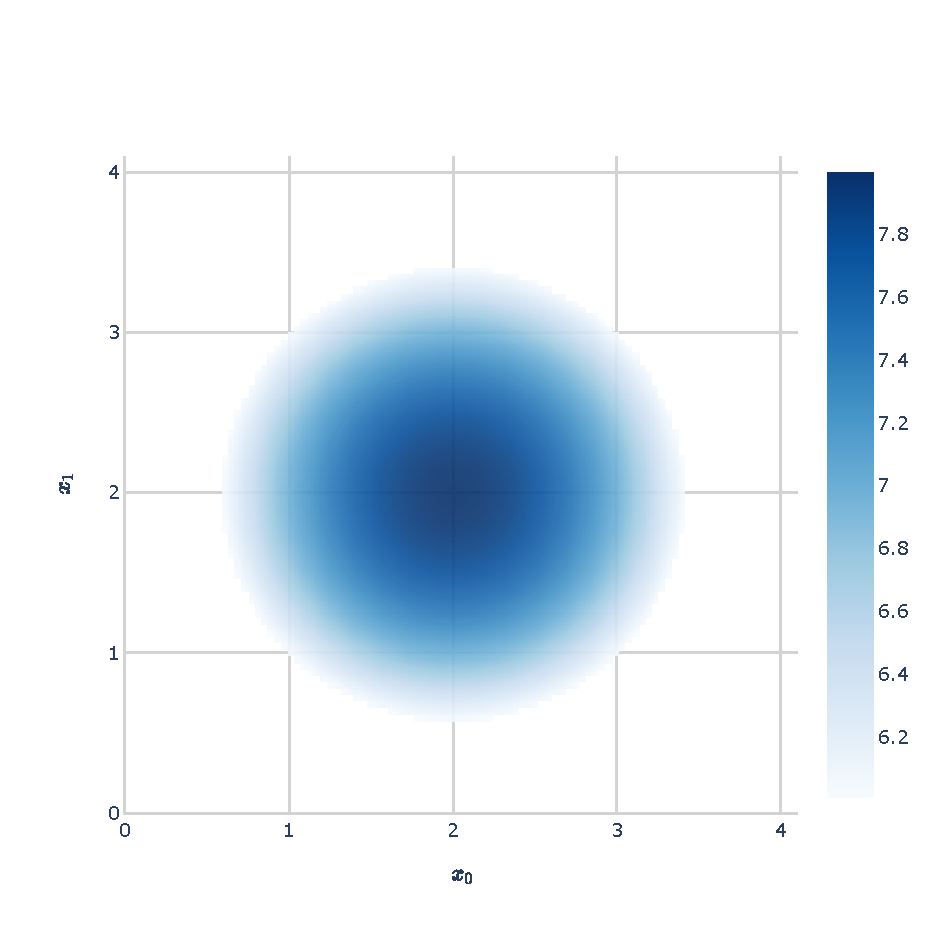
\includegraphics[width=0.5\textwidth]{contour-opt}
	\caption{
		\label{fig:g}
		Contour plot of $g$ defined in eq.~\eqref{eq:g}.
		Darker colors denote larger values, lighter colors denote smaller values.
		Values below $6$ are displayed as white.
	}
\end{figure}

In the bit basis, $g$ is implemented as
\begin{equation}
	M_{\alpha \beta}
        =
        - Q_{0\alpha}Q_{0\beta}
        - Q_{1\alpha}Q_{1\beta}
        + 4Q_{0\alpha}\delta_{\alpha\beta}
        + 4Q_{1\alpha}\delta_{\alpha\beta}
   \, , \qquad
   g(x_0, x_1) = \psi_\alpha M_{\alpha \beta} \psi_\beta + \vec b^2\, .
\end{equation}
This matrix is obtained by running \codeword{qlp.example.get_omega_0}.

We implement the following three constraints (see also fig. \ref{fig:constraints})
\begin{equation}
	\label{eq:constrained}
	0
	\leq
	f(\vec x)
	=
	\begin{cases}
		4 - x_0 - x_1 & (A) \\ 
		6 - x_0 - 3 x_1 & (B) \\
		3 - x_0 - x_1 & (C)
	\end{cases}
	\, .
\end{equation}

\begin{figure}
	\centering
	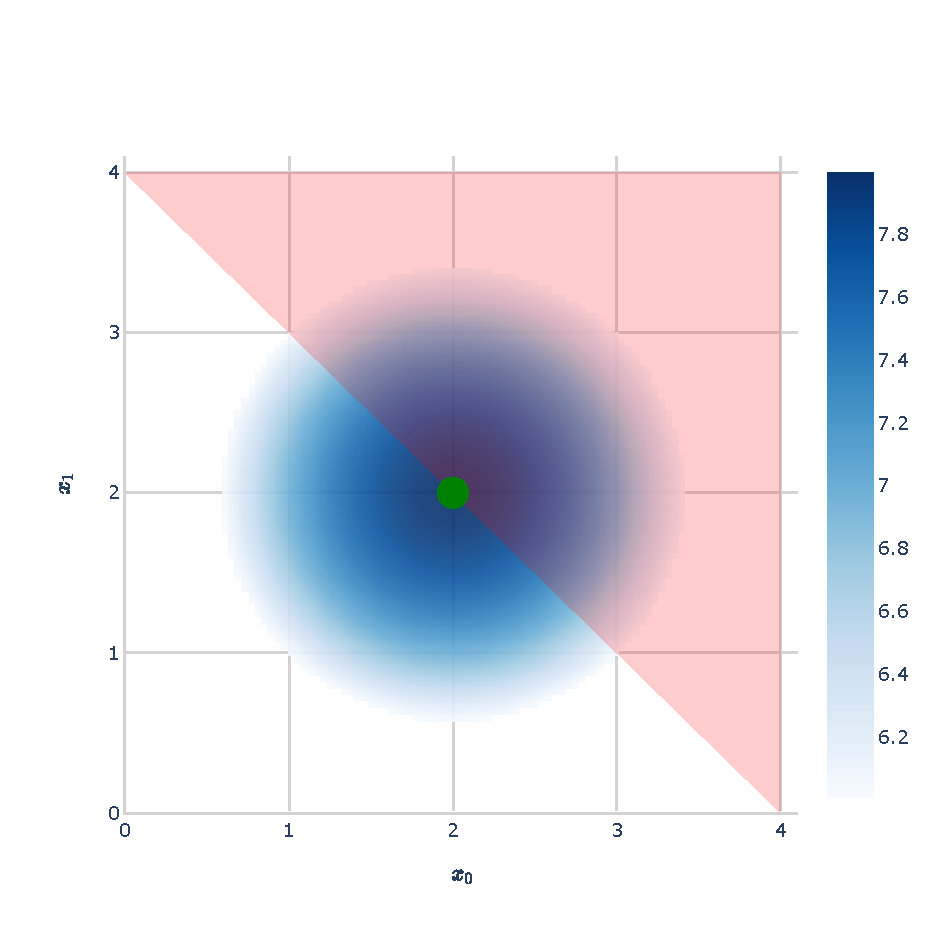
\includegraphics[width=0.32\textwidth]{contour-constraint-1}
	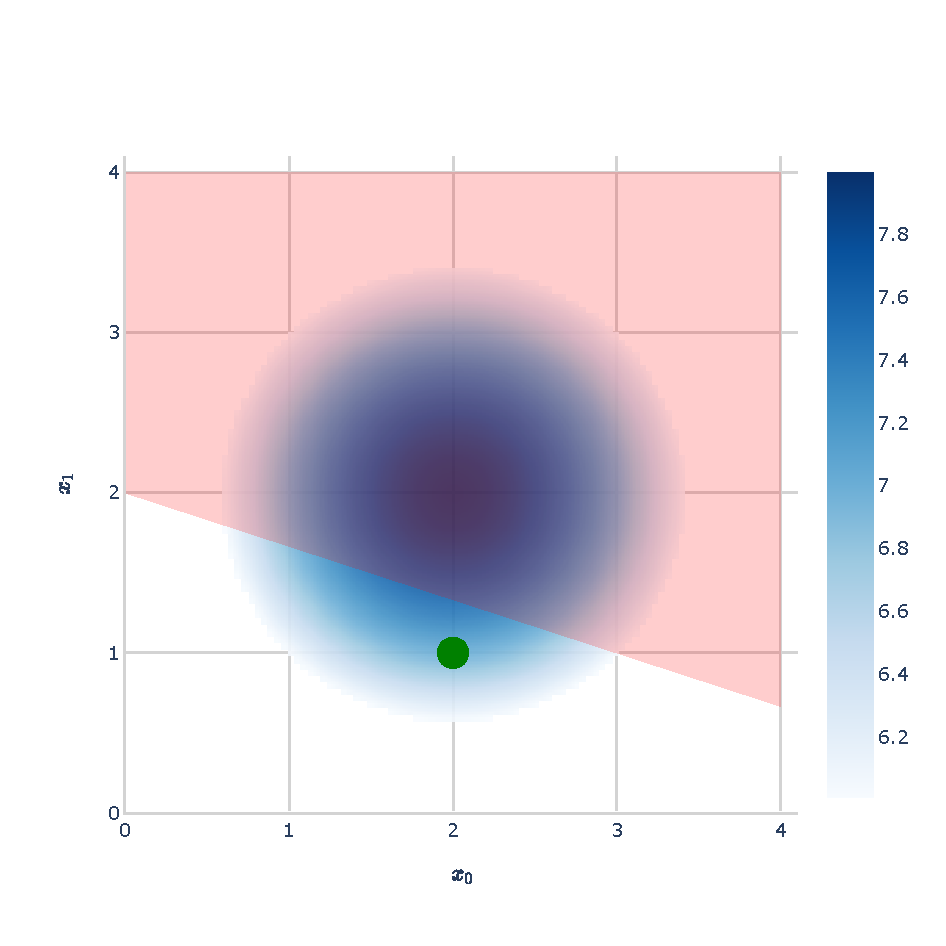
\includegraphics[width=0.32\textwidth]{contour-constraint-2}
	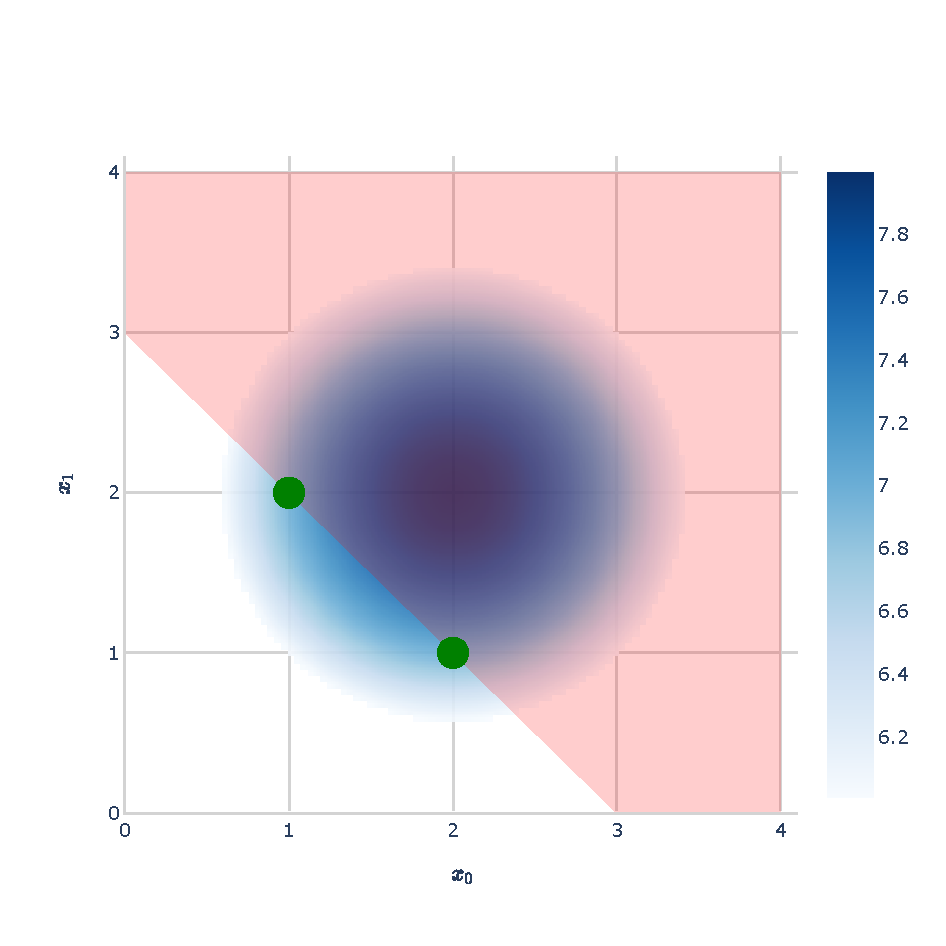
\includegraphics[width=0.32\textwidth]{contour-constraint-3}
	\caption{
		\label{fig:constraints}
		Contour plot of $g$ defined in eq.~\eqref{eq:g} with additional constraints (A), (B) and (C) defined in eq.~\eqref{eq:constrained}.
		The shaded red area displays the excluded space.
		Furthermore, $x_0, x_1 \geq 0$.
		The green dots display the location of the maximal value under the constraints.
		These values are obtained by running the \codeword{qlp} example problem.
		The constraint (A) does not change the location of the maximum, (B) shifts the maximum to a new value and (C) shifts the maximum and is degenerate.
	}
\end{figure}
The function \codeword{qlp.eqn_converter.constraints_to_matrix} converts a general list of inequalities to the matrix defined in eq.~\eqref{eq:constraint-matrix}.
This matrix does not contain the constant term $\vec b^2$.
Thus the vector-matrix-vector product can be negative and thus results in negative constraint values (increasing the total optimal maximization value).
However, for all bit vectors fulfilling the constraints, this negative value is the same and therefore does not influence the location of the optimal value.
To check this, we have implemented the methods \codeword{qlp.eqn_converter.generate_constrained_table}  (generating a table of all vector-matrix-vector operation results for all allowed bit vectors) and \codeword{qlp.checks.run_checks} to check the consistency of the generated tables. 
 
The full matrix including the constraints is obtained by running \codeword{qlp.example.get_omega}~.
Similar to the checks we run \codeword{qlp.eqn_converter.generate_table} to probe the full bit space and pick the maximal value (displayed in fig.~\ref{fig:constraints}).

The example is presented in the notebook \codeword{notebooks/example-problem.ipynb}.
To use this notebook, you have to run \codeword{pip install [--user] -e .} in the repo root directory first.

\end{document}
